\section{Coincidence Time}
The \textit{coincidence time} is the difference between the trigger time
recorded by one spectrometer and the trigger time recorded by the other
spectrometer.
The TDC times recorded in Hall C are precise enough that a histogram of
coincidence times will show of a series of peaks separated by
\SI{2}{\nano\second}, reflecting the CEBAF beam bunching structure.
In addition, a given pair of spectrometer central momenta will show different
types of scattering events (e.g. $ep$, $e\pi^+$, $\pi^-\pi^+$, ...) lying in
different coincidence time peaks; the differing particle masses result in
differing velocities for a given momentum.

% TODO: Clarify coincidence TDC start/top
Given single arm TDC trigger times $t^H$ and $t^P$ and coincidence TDC trigger
time $t^{coin}$, the uncorrected coincidence time is
\begin{equation}
    t^{coin}_{uncorrected} = t^H - t^P - t^{coin}
\end{equation}

Using the particles' velocities, models of the spectrometers' optics, and
surveys of Hall C, these times are corrected for the additional time it takes a
particle not traveling along the central ray of a spectrometer.
Given $x'_{tar}$ in \si{\milli\radian} and $\delta$ in percent, the additional
length traveled is given by
\begin{align}
    \Delta L^P &= 0.11 * x'^{P}_{tar} * 1000 + 0.057 * \delta^{P}/100 \\
    \Delta L^H &= 0.12 * x'^{H}_{tar}* 1000 + 0.17 * \delta^{H}/100
\end{align}

Let $v$ be a particle's velocity\footnote{Given reconstructed momentum $p$, a
 particle has velocity $\beta = v/c = p / \sqrt{p^2+m^2}$.},
$L^{P(H)}$ the length of the the central ray of the SHMS (HMS),
$\Delta L^{P(H)}$ the additional length traveled beyond the central ray,
$\langle t^{P(H)}_{hodostart}\rangle$ the hodoscope start time, and
$t^{P(H)}_{fp}$ the focal plane time.
% TODO: footnote reminding us of the definitions of these times
Then the SHMS (HMS) correction $\Delta t^{P(H)}$ is
\begin{align}
    \Delta t^P &= \frac{L^P}{v} + \frac{\Delta L^P}{v} + \left( \langle t^{P}_{hodostart}\rangle - t^{P}_{fp} \right) \\
    \Delta t^H &= \frac{L^H}{v} + \frac{\Delta L^H}{v} + \left( \langle t^{H}_{hodostart}\rangle - t^{H}_{fp} \right)
\end{align}

The corrected coincidence time is
\begin{equation}
    t^{coin}_{corrected} = (t^P - \Delta t^P) - (t^H - \Delta t^H) - t_{offset}
\end{equation}
where $t_{offset}$ is an offset due to signal propagation times which can be
corrected for in PARAM files if desired.
Strictly speaking, this is not necessary, because one identifies the location of
the true coincidence peak in the coincidence time spectrum and places cuts
around this value, whether or not it's centered at zero.

Coincidence time distributions for two runs are shown in
Fig~\ref{fig:cointime}.
The distribution on the left comes from a run with large backgrounds,
which result in numerous peaks in coincidence time.
A large peak corresponding true $ep$ coincidences can be seen near \SI{0}{\nano\second},
and a smaller peak corresponding to $e\pi^+$ coincidences to the left near
\SI{-5}{\nano\second}.
The smaller peaks separated by \SI{4}{\nano\second} are accidental coincidences
coming from other beam bunches.
The distribution on the right is a typical run from this experiment and shows
negligible contributions from accidental coincidences.

\begin{figure}[ht]
    \centering
    \begin{subfigure}[b]{0.45\textwidth}
        \centering
        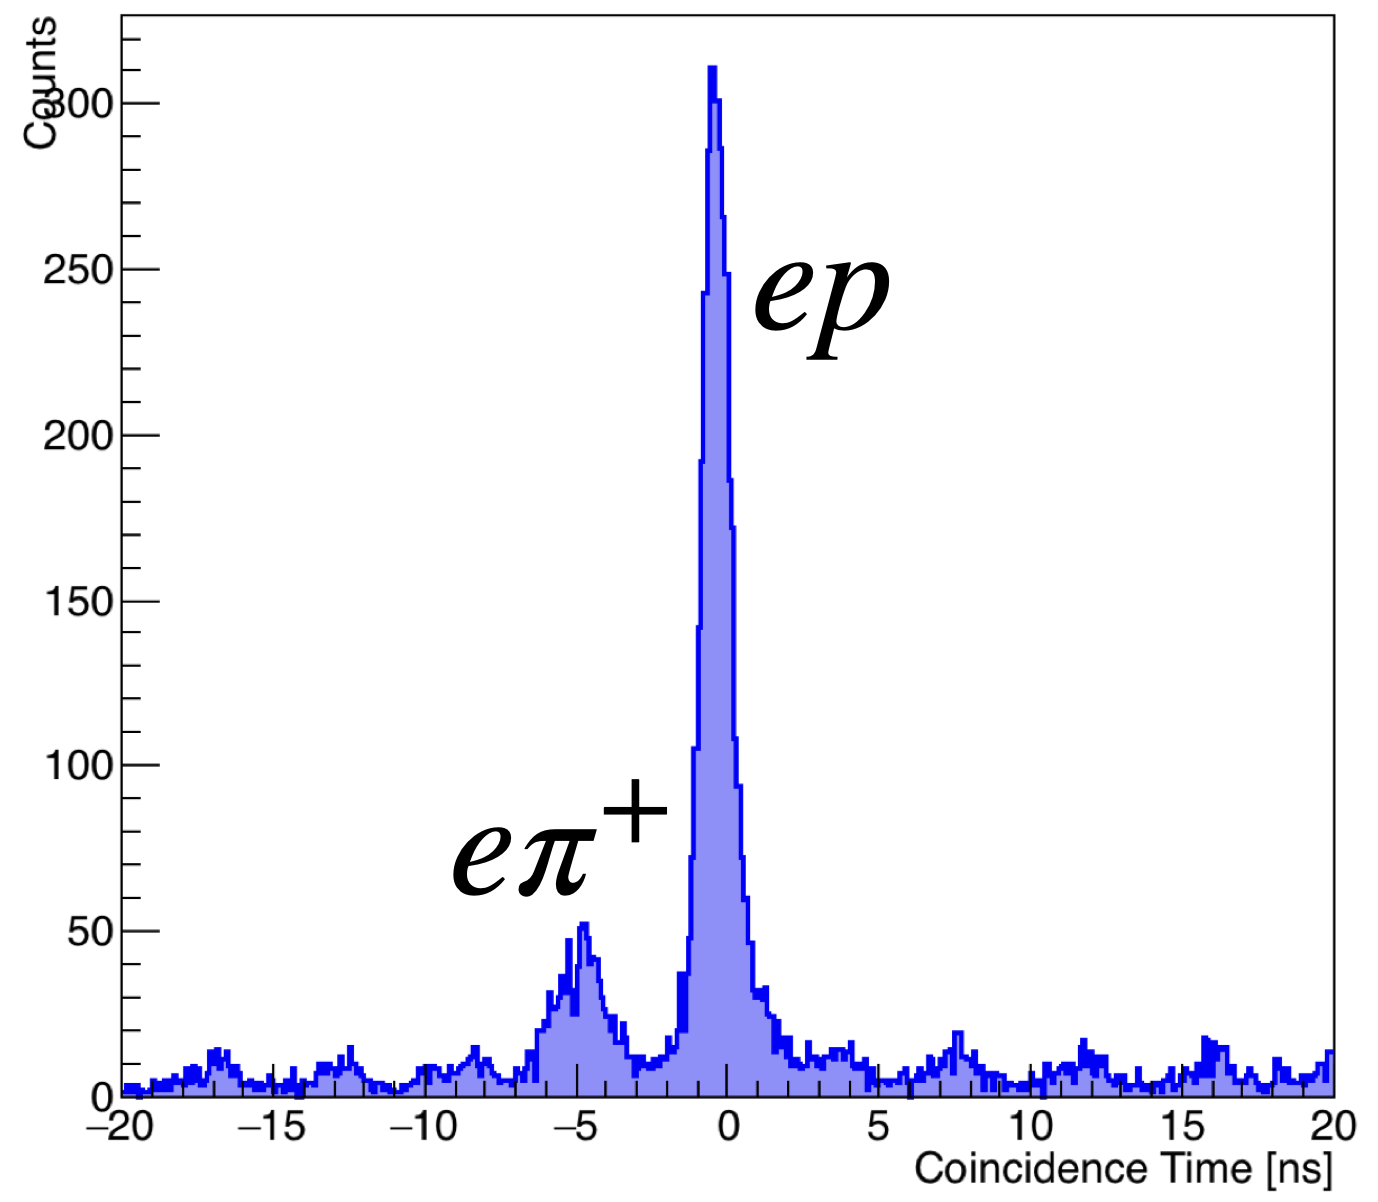
\includegraphics[height=6cm]{chap4/cointime_dirty.png}
        \caption{To coincidence time distribution for a run taken specifically to
                 observe the structure caused by different coincidence types.}
        \label{fig:cointime_dirty}
    \end{subfigure}
    \hfill
    \begin{subfigure}[b]{0.45\textwidth}
        \centering
        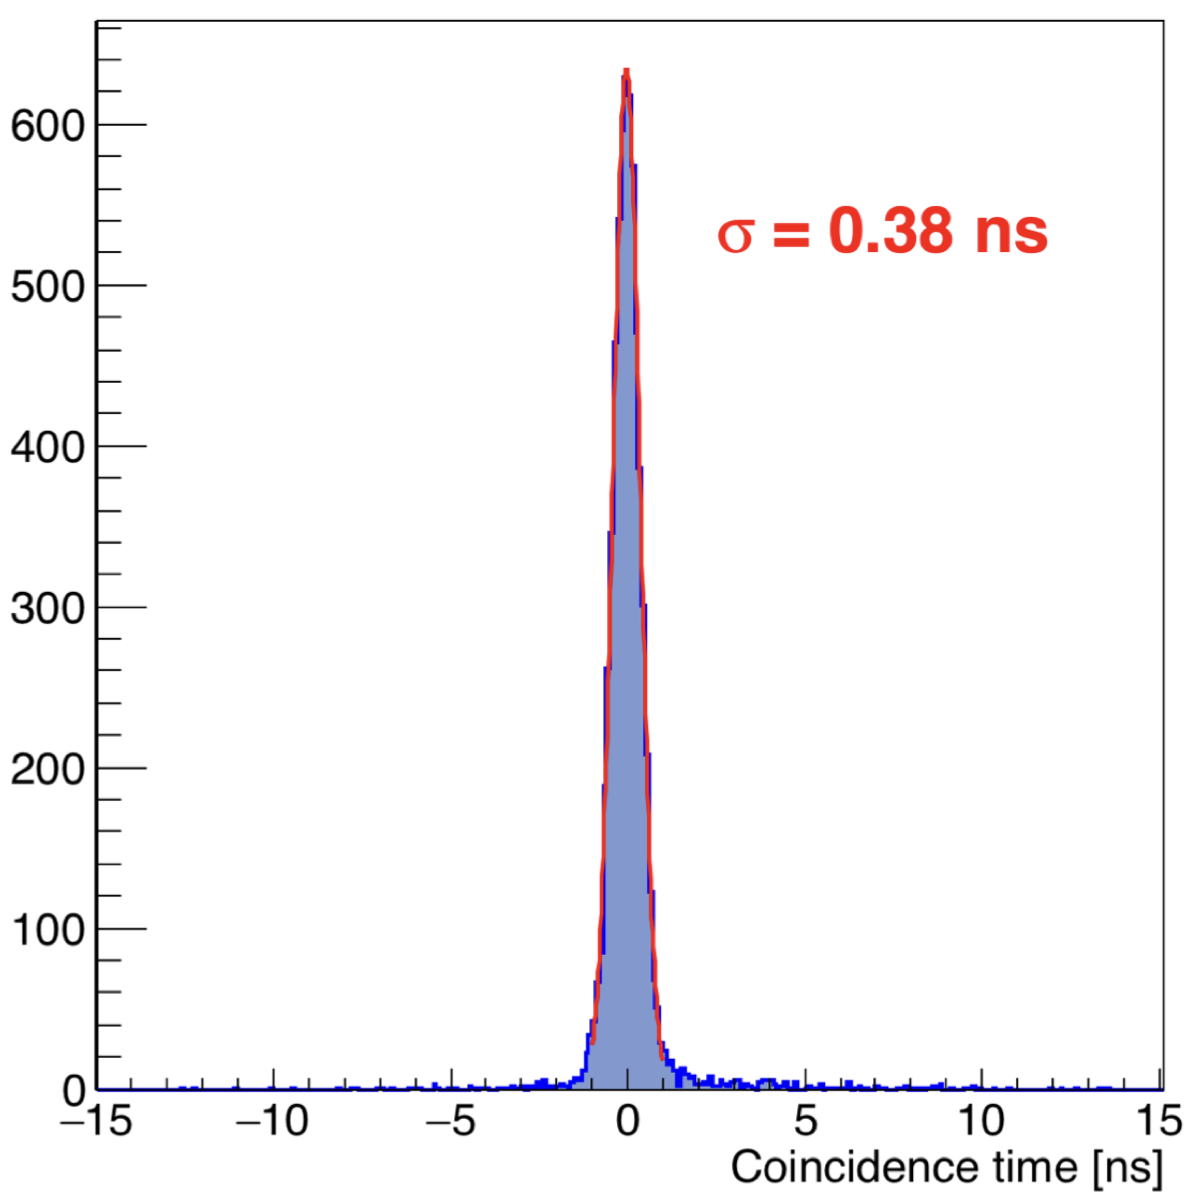
\includegraphics[height=6cm]{chap4/cointime_clean.png}
        \caption{The coincidence time distribution for a typical production run
                 is very clean, with negligible accidental coincidences.}
        \label{fig:cointime_clean}
    \end{subfigure}
    \caption{The distribution of coincidence times for two runs.}
    \label{fig:cointime}
\end{figure}

